% \documentclass[aspectratio=169,notes]{beamer}
\documentclass[aspectratio=169]{beamer}
\usetheme[faculty=phil]{fibeamer}
\usepackage{polyglossia}
\setmainlanguage{english} %% main locale instead of `english`, you
%% can typeset the presentation in either Czech or Slovak,
%% respectively.
\setotherlanguages{russian} %% The additional keys allow
%%
%%   \begin{otherlanguage}{czech}   ... \end{otherlanguage}
%%   \begin{otherlanguage}{slovak}  ... \end{otherlanguage}
%%
%% These macros specify information about the presentation
\title[AGLA1]{Analytical Geometry and Linear Algebra I, Lab 4} %% that will be typeset on the
\subtitle{Inverse Matrix \\ Change of basis \\ \    
         } %% title page.
\author{Oleg Bulichev}
%% These additional packages are used within the document:
\usepackage{ragged2e}  % `\justifying` text
\usepackage{booktabs}  % Tables
\usepackage{tabularx}
\usepackage{tikz}      % Diagrams
\usetikzlibrary{calc, shapes, backgrounds}
\usepackage{amsmath, amssymb}
\usepackage{url}       % `\url`s
\usepackage{listings}  % Code listings
% \usepackage{subfigure}
\usepackage{floatrow}
\usepackage{subcaption}
\usepackage{mathtools}
\usepackage{todonotes}
\usepackage{fontspec}
\usepackage{multicol}
\usepackage{pdfpages}
\usepackage{wrapfig}
\usepackage{animate}
\usepackage{booktabs}
\usepackage{multirow}

\graphicspath{{resources/}}
\frenchspacing

\setbeamertemplate{caption}[numbered]
\usetikzlibrary{graphs}

% \usepackage[backend=biber,style=ieee,autocite=footnote]{biblatex}
% \addbibresource{biblio.bib}
% \DefineBibliographyStrings{english}{%
%   bibliography = {References},}

\newcommand{\oleg}[2][] {\todo[color=red, #1] {OLEG:\\ #2}}
\newcommand{\fbckg}[1]{\usebackgroundtemplate{\includegraphics[width=\paperwidth]{#1}}}%frame background

\usepackage[framemethod=TikZ]{mdframed}
\newcommand{\dbox}[1]{
\begin{mdframed}[roundcorner=3pt, backgroundcolor=yellow, linewidth=0]
\vspace{1mm}
{#1}
\vspace{1mm}
\end{mdframed}
}

\begin{document}
\setlength{\abovedisplayskip}{0pt}
\setlength{\belowdisplayskip}{0pt}
\setlength{\abovedisplayshortskip}{0pt}
\setlength{\belowdisplayshortskip}{0pt}

\fbckg{fibeamer/figs/title_page.png}
\frame[c]{\setcounter{framenumber}{0}
    \usebeamerfont{title}%
    \usebeamercolor[fg]{title}%
    \begin{minipage}[b][6.5\baselineskip][b]{\textwidth}%
        \textcolor{black}{\raggedright\inserttitle}
    \end{minipage}
    % \vskip-1.5\baselineskip

    \usebeamerfont{subtitle}%
    \usebeamercolor[fg]{framesubtitle}%
    \begin{minipage}[b][3\baselineskip][b]{\textwidth}
        \raggedright%
        \insertsubtitle%
    \end{minipage}
    \vskip.25\baselineskip
}
%   \frame[c]{\maketitle}
\note{
    \begin{enumerate}
        \item Смену базиса давать через вывод формулы: вектор - фреймлесс, а координаты вектора - нет. Поэтому можно вот выразить ручку по разному. Все на основе линейных комбинаций. \smallskip

              Есть 2 твои формулы - бро $E' = EA$ и $Ex=E'x'$. Разновидность бро $Ex = Eb + E'x'$, где $E = [e_1\ e_2\ e_3]$, $E = [e'_1\ e'_2\ e'_3]$

        \item Забить на слайды и объяснять на маркерах, ручках и доске про смену базиса

    \end{enumerate}
}

\fbckg{fibeamer/figs/common.png}


\begin{frame}[c]{Questions from the class}
    \framesubtitle{}
    \centering
    \textit{ \Large No questions for today}
\end{frame}

\begin{frame}[t]{Inverse Matrix}
    \framesubtitle{What is it?}
    \textbf{Inverse matrix} $A^{-1}$ is the matrix, the product of which to original matrix $A$ is equal to the \textit{identity matrix} $I$:

    \begin{equation*}
        A \cdot A^{-1} = A^{-1} \cdot A = I
    \end{equation*}
\end{frame}

\note{Доказать им, что это работает формула, тут \href{https://www.berdov.com/works/matrix/obratnaya-matrica/}{подсказка} (Лемма 2, 13 минута)}

\begin{frame}[t]{Inverse Matrix}
    \framesubtitle{Why do we need it?}
    \vspace{-3ex}
    \begin{figure}[H]
        \centering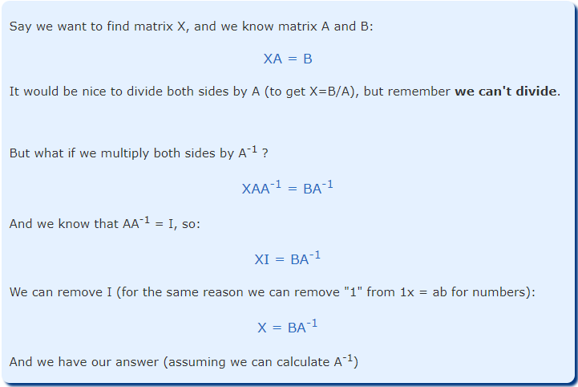
\includegraphics[height=6cm,width=1\textwidth,keepaspectratio]{inverse_why.png}
        % \caption{caption_name}
        \label{fig:inverse_why.png}
    \end{figure}
\end{frame}

\begin{frame}[t]{Inverse Matrix}
    \framesubtitle{Properties}
    \begin{enumerate}
        \item $det(A^{-1}) = \dfrac{1}{det(A)}$
        \item $(AB)^{-1}=A^{-1}B^{-1}$
        \item $(A^{-1})^T=(A^T)^{-1}$
        \item $(kA)^{-1}=\dfrac{A^{-1}}{k}$
        \item $(A^{-1})^{-1}=A$
    \end{enumerate}
\end{frame}

\begin{frame}[t]{Inverse Matrix}
    \framesubtitle{How to find}
    There are 2 ways:
    \begin{enumerate}
        \item Classical approach
        \item Gauss-Jordan / Reduced Row Echelon Form (RREF)
    \end{enumerate}
\end{frame}

\begin{frame}[t]{Inverse Matrix: Classical Approach}
    \framesubtitle{Theory}
    $\underset{2 \times 2}{A}^{-1} = \dfrac{C^T}{det(A)}$, where $C$ is a matrix of \textit{cofactors}. \smallskip

    $\underset{2 \times 2}{C} = \begin{bmatrix} C_{11} & C_{12} \\ C_{21} & C_{22} \end{bmatrix}$, where $C_{ij} = (-1)^{i+j}M_{ij}$ --- (we met it on previous lab (lab 3))
\end{frame}

\begin{frame}[t]{Inverse Matrix: Classical Approach}
    \framesubtitle{Case Study}
    \vspace{-0.5cm}
    \begin{multicols}{2}
        $A=\begin{bmatrix}
                1 & 2 \\
                3 & 4
            \end{bmatrix}$. Let's find $A^{-1}$.
        \begin{enumerate}
            \item Find a determinant (shouldn't be equal to $0$, otherwise $\rightarrow$ stop calculations).

                  $det(A)=1 \cdot 4 - 2 \cdot 3 = -2$
            \item Find Cofactor matrix
                  $C_{11} = (-1)^{1+1}M_{11}=(-1)^2|4|=4$\\
                  $C_{12} = (-1)^{1+2}M_{12}=(-1)^3|3|=-3$\\
                  $C_{21} = (-1)^{2+1}M_{21}=(-1)^3|2|=-2$\\
                  $C_{22} = (-1)^{2+2}M_{22}=(-1)^4|1|=1$\\
                  $C = \begin{bmatrix} 4 & -3\\ -2 & 1\end{bmatrix}$
            \item Transpose cofactor matrix\\
                  $C^T=\begin{bmatrix} 4 & -2\\ -3 & 1\end{bmatrix}$
            \item Substitute it to the main formula \medskip

                  $A^{-1}=\dfrac{\begin{bmatrix} 4 & -2\\ -3 & 1\end{bmatrix}}{-2} = \begin{bmatrix} -2 & 1\\ 1.5 & -0.5\end{bmatrix}$
        \end{enumerate}
    \end{multicols}
\end{frame}

\begin{frame}[t]{Inverse Matrix: Gauss-Jordan}
    \framesubtitle{Core Idea for Inverse Matrices}
    \vspace{-0.4cm}
    $(A|I)\rightarrow \ldots \rightarrow (I|A^{-1})$
    \begin{enumerate}
        \item Using sequence of \textit{elementary row operations} to modify the matrix until the lower left-hand corner of the matrix is filled with zeros (\textbf{Row Echelon Form}/Upper Trianglular Matrix). $(A|I)\rightarrow \ldots \rightarrow (\lhd_{Upper} |B)$
        \item Using \textit{elementary row operations} transform Upper Trianglular Matrix to Indentity Matrix. $(\lhd_{Upper} |B)\rightarrow \ldots \rightarrow (I|A^{-1})$
    \end{enumerate}
    \begin{exampleblock}{Elementary Row Operations}
        \vspace{-0.5cm}
        \begin{multicols}{2}
            \begin{itemize}
                \item Swapping two rows,
                \item Multiplying a row by a nonzero number,
                \item Adding a multiple of one row to another row. (subtraction can be achieved by multiplying one row with -1 and adding the result to another row)
            \end{itemize}
        \end{multicols}
    \end{exampleblock}

\end{frame}

\note{Объяснить надо, что такое чёрточка (там прячутся неизвестные). И подвести все к системам уравнений

    Спросить про уникальность верхнего треугольника и редьюсед формы}

\begin{frame}[t]{Inverse Matrix: Gauss-Jordan}
    \framesubtitle{Case study ($2 \times 2$)}
    \vspace{-0.6cm}
    \begin{figure}[H]
        \centering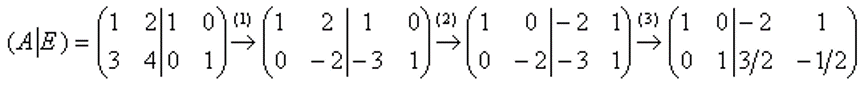
\includegraphics[height=6cm,width=1\textwidth,keepaspectratio]{Gauss2x2.png}
        % \caption{caption_name}
        \label{fig:Gauss2x2.png}
    \end{figure}
\end{frame}

\begin{frame}[t]{Inverse Matrix: Gauss-Jordan}
    \framesubtitle{Case study ($4 \times 4$)}
    \vspace{-0.6cm}
    \begin{figure}[H]
        \centering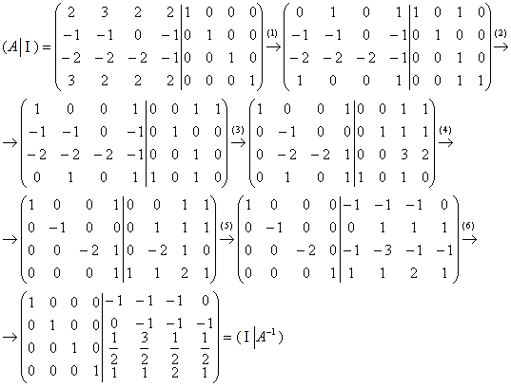
\includegraphics[height=6cm,width=1\textwidth,keepaspectratio]{Gauss4x4.png}
        % \caption{caption_name}
        \label{fig:Gauss4x4.png}
    \end{figure}
\end{frame}

\begin{frame}[t]{Inverse Matrix}
    \framesubtitle{Task 1}
    Find inverse matrices for the following matrices:
    \begin{enumerate}

        \item $\begin{bmatrix}
                      3 & 5 \\
                      5 & 9 \\
                  \end{bmatrix}$;
        \item $\begin{bmatrix}2&-1&0\\0&2&-1\\-1&-1&1\end{bmatrix}$;
    \end{enumerate}
\end{frame}

\begin{frame}[t]{Inverse Matrix}
    \framesubtitle{Task 2}
    Solve matrix equations:
    \begin{enumerate}
        \item $\begin{bmatrix}2&5\\1&3\end{bmatrix}X=\begin{bmatrix}2&1\\1&1\end{bmatrix}$;
        \item  $X\begin{bmatrix}2&5\\1&3\end{bmatrix}=\begin{bmatrix}2&1\\1&1\end{bmatrix}$;
    \end{enumerate}
\end{frame}

\begin{frame}[t]{}
    \framesubtitle{}
    \begin{figure}[H]
        \centering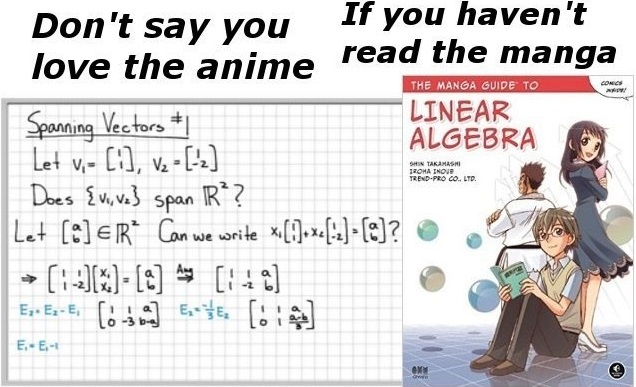
\includegraphics[height=7cm,width=1\textwidth,keepaspectratio]{agla_manga.jpeg}
        % \caption{caption_name}
        \label{fig:agla_manga.jpeg}
    \end{figure}
\end{frame}


\begin{frame}[t]{Preparation to Exam / Test}
    \framesubtitle{Strategy for efficient exam solving}
    \begin{exampleblock}{Problem Statement}
        During an exam, I \textit{spend too much time} on finding the solution
    \end{exampleblock}
    \begin{alertblock}{Solution}
        To find the right strategy for \textit{preparation} and \textit{behavior} during an exam.
    \end{alertblock}
\end{frame}

\begin{frame}[t]{Preparation to Exam / Test}
    \framesubtitle{My own guide and thoughts}
    \textbf{ I should pay attention on this parts:}
    \begin{enumerate}
        \item Preparation before a test
        \item Preparation in a day of a test
        \item Behavior on exam
    \end{enumerate}

    \textbf{Approx time consuming:}
    \begin{itemize}
        \item Preparation: 3-8 hours in overall
        \item Exam: \begin{itemize}
                  \item Find the idea how to solve a particular task --- 10 sec - 2 min
                  \item Implement the idea — 10-20 min
              \end{itemize}
    \end{itemize}
\end{frame}

\begin{frame}[t]{Preparation to Exam / Test}
    \framesubtitle{Preparation strategy}
    \vspace{-0.7cm}
    \begin{columns}[T,onlytextwidth]
        \begin{column}{0.59\textwidth}
            \begin{enumerate}
                \item Understand the concept of a new topic \\ (\underline{Apply} or \underline{Analyze} in terms of Bloom's Taxonomy)
                      \begin{enumerate}
                          \item Look at slides and videos
                          \item Play with concept (suggest some ideas and prove it or disprove via computer or hand calculations)
                      \end{enumerate}
                \item Take a book (material) with exercises and solutions for it. \begin{enumerate}
                          \item Look at a task, imagine how to solve it.
                          \item Check a suggestion from solutions. If you sure that your solution is also applicable --- check it.
                      \end{enumerate}
            \end{enumerate}
            \alert{Important}: For some tasks \textit{practical skills} are crutial (find not only an idea, but implement it)!
        \end{column}
        \begin{column}{0.39\textwidth}
            \begin{figure}[H]
                \centering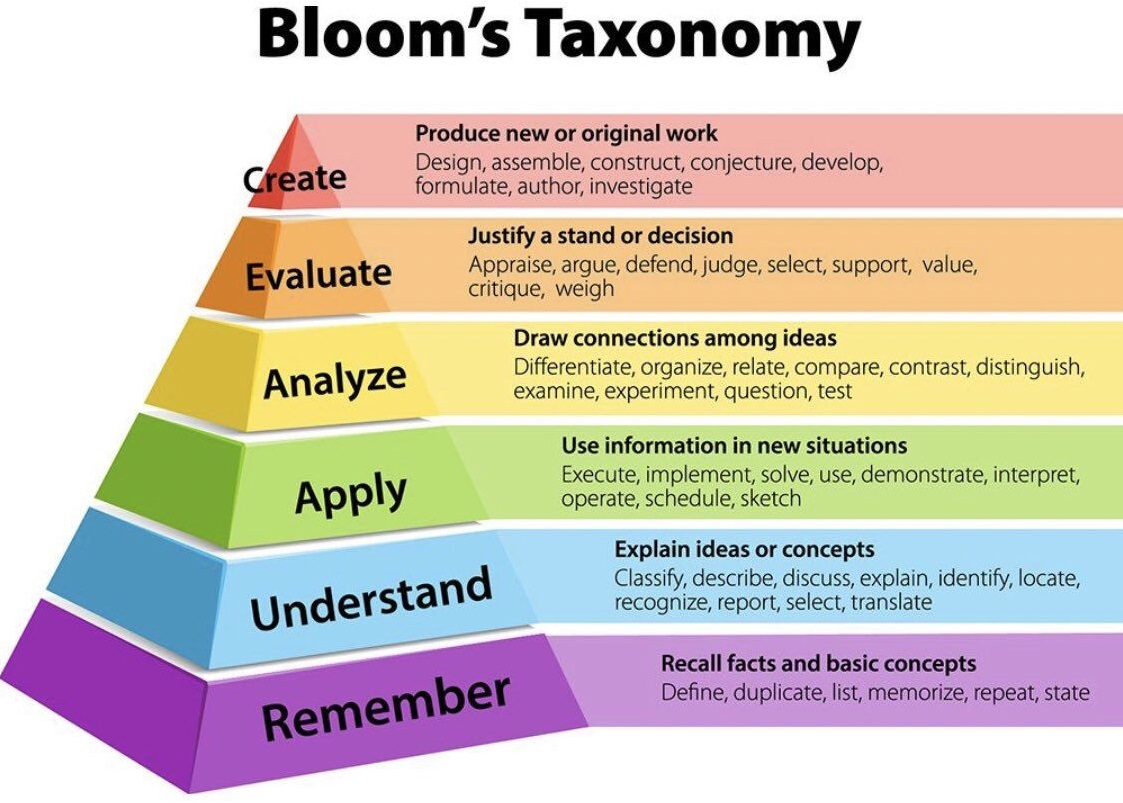
\includegraphics[height=6cm,width=1\textwidth,keepaspectratio]{bloom_taxonomy.png}
                % \caption{caption_name}
                \label{fig:bloom_taxonomy.png}
            \end{figure}
        \end{column}
    \end{columns}
\end{frame}

\begin{frame}[t]{Preparation to Exam / Test}
    \vspace{-0.5cm}
    \framesubtitle{Behavior before and on exam}
    \textbf{Before}:

    Prepare your brain (skim the material) and mentality (by self hypnosis techniques) \\ (took from science russian book \href{https://yadi.sk/d/uZhNSQW637Q3v7}{"Преодолей себя! Психическая подготовка в спорте"}) \smallskip

    \textbf{During an exam}:
    \begin{enumerate}
        \item Rank tasks by doing speed: \begin{itemize}
                  \item Can be solved on-a-fly (expect max grade)
                  \item Easy concept --- tough implementation (expect that some computational mistakes can be done)
                  \item Tough concept (cannot find the solution on-a-fly) (time consuming tasks)
              \end{itemize}
        \item Solve it in such order
        \item Profit! You are awesome!
    \end{enumerate}
\end{frame}

\begin{frame}[t]{Changing Basis}
    \framesubtitle{Case Study: Shoe Polishing Robot}
    \vspace{-0.6cm}
    \begin{figure}[H]
        \centering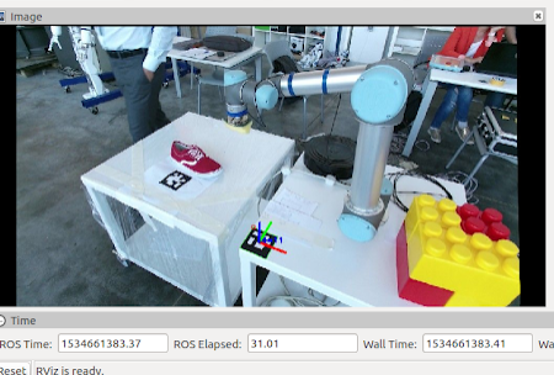
\includegraphics[height=6cm,width=1\textwidth,keepaspectratio]{change_basis_practice_2.png}
        % \caption{caption_name}
        \label{fig:change_basis_practice_2.png}
    \end{figure}
\end{frame}

\begin{frame}[t]{Changing Basis}
    \framesubtitle{Case Study: Shoe Polishing Robot, How it works}
    \vspace{-0.6cm}
    \begin{figure}[H]
        \centering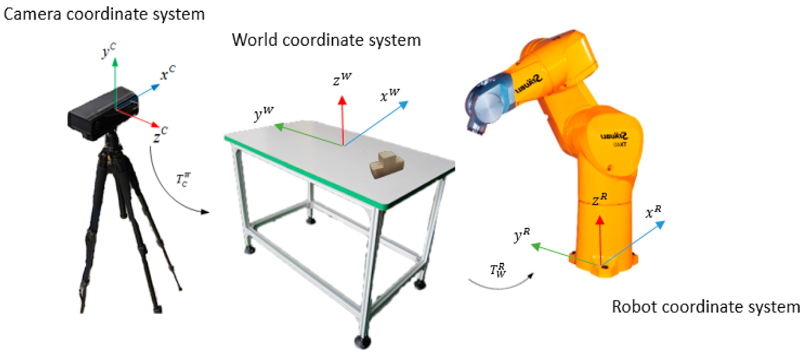
\includegraphics[height=6cm,width=1\textwidth,keepaspectratio]{change_basis_practice_1.png}
        % \caption{caption_name}
        \label{fig:change_basis_practice_1.png}
    \end{figure}
\end{frame}

\begin{frame}[t]{Changing Basis}
    \framesubtitle{Two Bros in the World of Changing Basis}
    \LARGE \centering$E' = EA$ and $Ex=E'x'$.

    Extended Bro Equation: $Ex = Eb + E'x'$, where $E = [e_1\ e_2\ e_3] = \begin{bmatrix}e_{1x}\\e_{1y} \\ e_{1z}\end{bmatrix},\ \begin{bmatrix}e_{2x}\\e_{2y} \\ e_{2z}\end{bmatrix},\ \begin{bmatrix}e_{3x}\\e_{3y} \\ e_{3z}\end{bmatrix}$, $E' = [e'_1\ e'_2\ e'_3]$ \smallskip

    More info in Appendix \ref{pdf:myfile}
\end{frame}

\usebackgroundtemplate{}
\setbeamercolor{background canvas}{bg=}
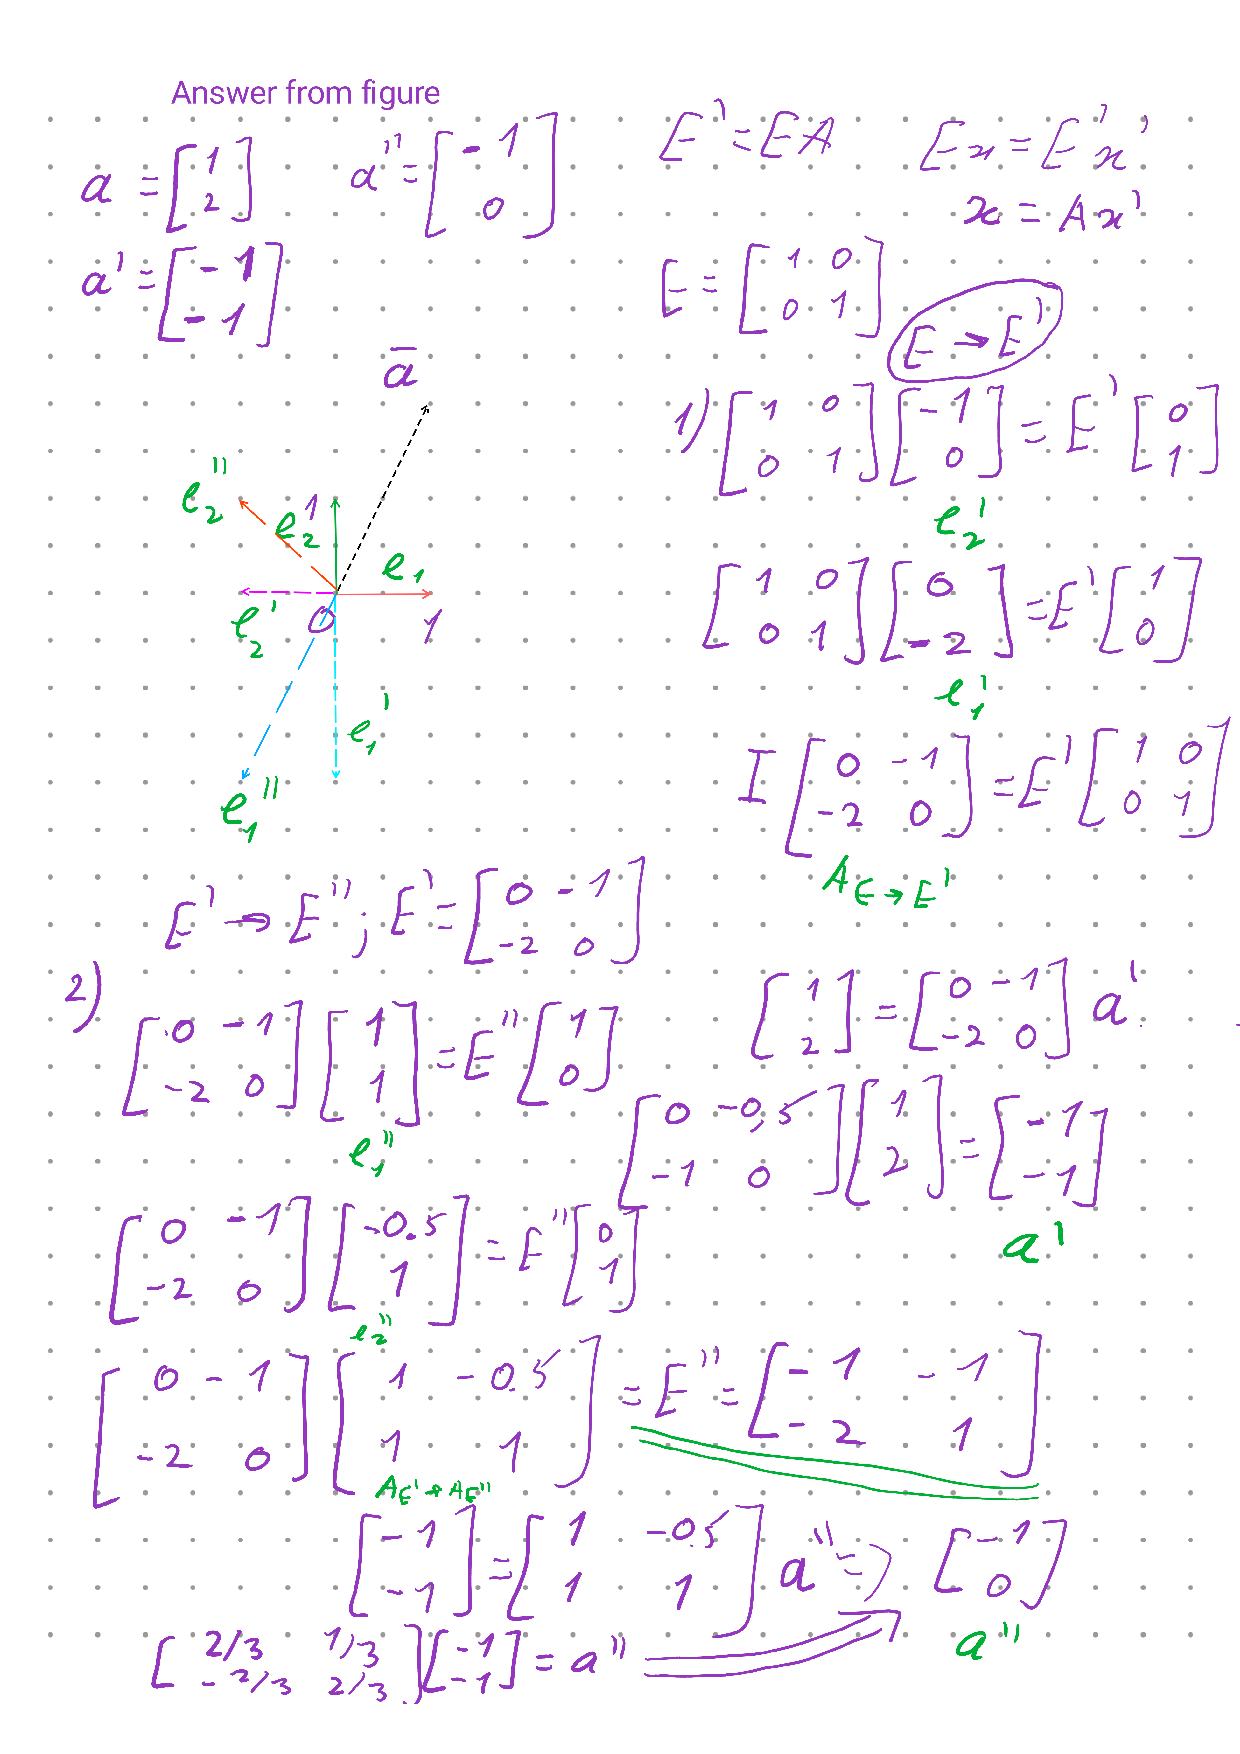
\includepdf[pages=-,fitpaper, linktodoc=true, pagecommand={\section{two_bros}\label{pdf:two_bros}}]{two_bros_fig.pdf}
\fbckg{fibeamer/figs/common.png}

\begin{frame}[t]{Changing Basis}
    \framesubtitle{Task 3}
    \only<1>{If vectors \textbf{a} and \textbf{b} form a basis (you should check it), it is needed to find coordinates $\textbf{c}$ in the basis.\medskip

    $\textbf{a}=\begin{bmatrix} -5 \\ -1 \end{bmatrix}$, $\textbf{b}=\begin{bmatrix} -1 \\ 3\end{bmatrix}$,
    $\textbf{c}=\begin{bmatrix} -1 \\ 2 \end{bmatrix}$.}
    \only<2>{\alert{\Large Answer}

    \begin{align*}
        E = \begin{bmatrix}
        1 & 0\\ 
        0 & 1 
        \end{bmatrix},\ E' = \begin{bmatrix}
        -5 & -1\\ 
        -1 & 3 
        \end{bmatrix} \\
        \text{Because we are interested in coordinates, 2nd bro} \\
        Ec_{old} = E'x \rightarrow \begin{bmatrix}
            1 & 0\\ 
            0 & 1 
            \end{bmatrix}\begin{bmatrix} -1\\ 2 \end{bmatrix} = \begin{bmatrix}
            -5 & -1\\ 
            -1 & 3 
            \end{bmatrix}\begin{bmatrix} c_{new_x}\\c_{new_y} \end{bmatrix} \\
            \begin{bmatrix} c_{new_x}\\c_{new_y} \end{bmatrix} = (E')^{-1}c_{old} = \begin{bmatrix} \frac{1}{16}\\ \frac{11}{16} \end{bmatrix}
    \end{align*}
    }
    \only<3>{
        \vspace{-0.6cm}
        \begin{figure}[H]
            \href{https://www.geogebra.org/calculator/zyamrfcn}{
                \centering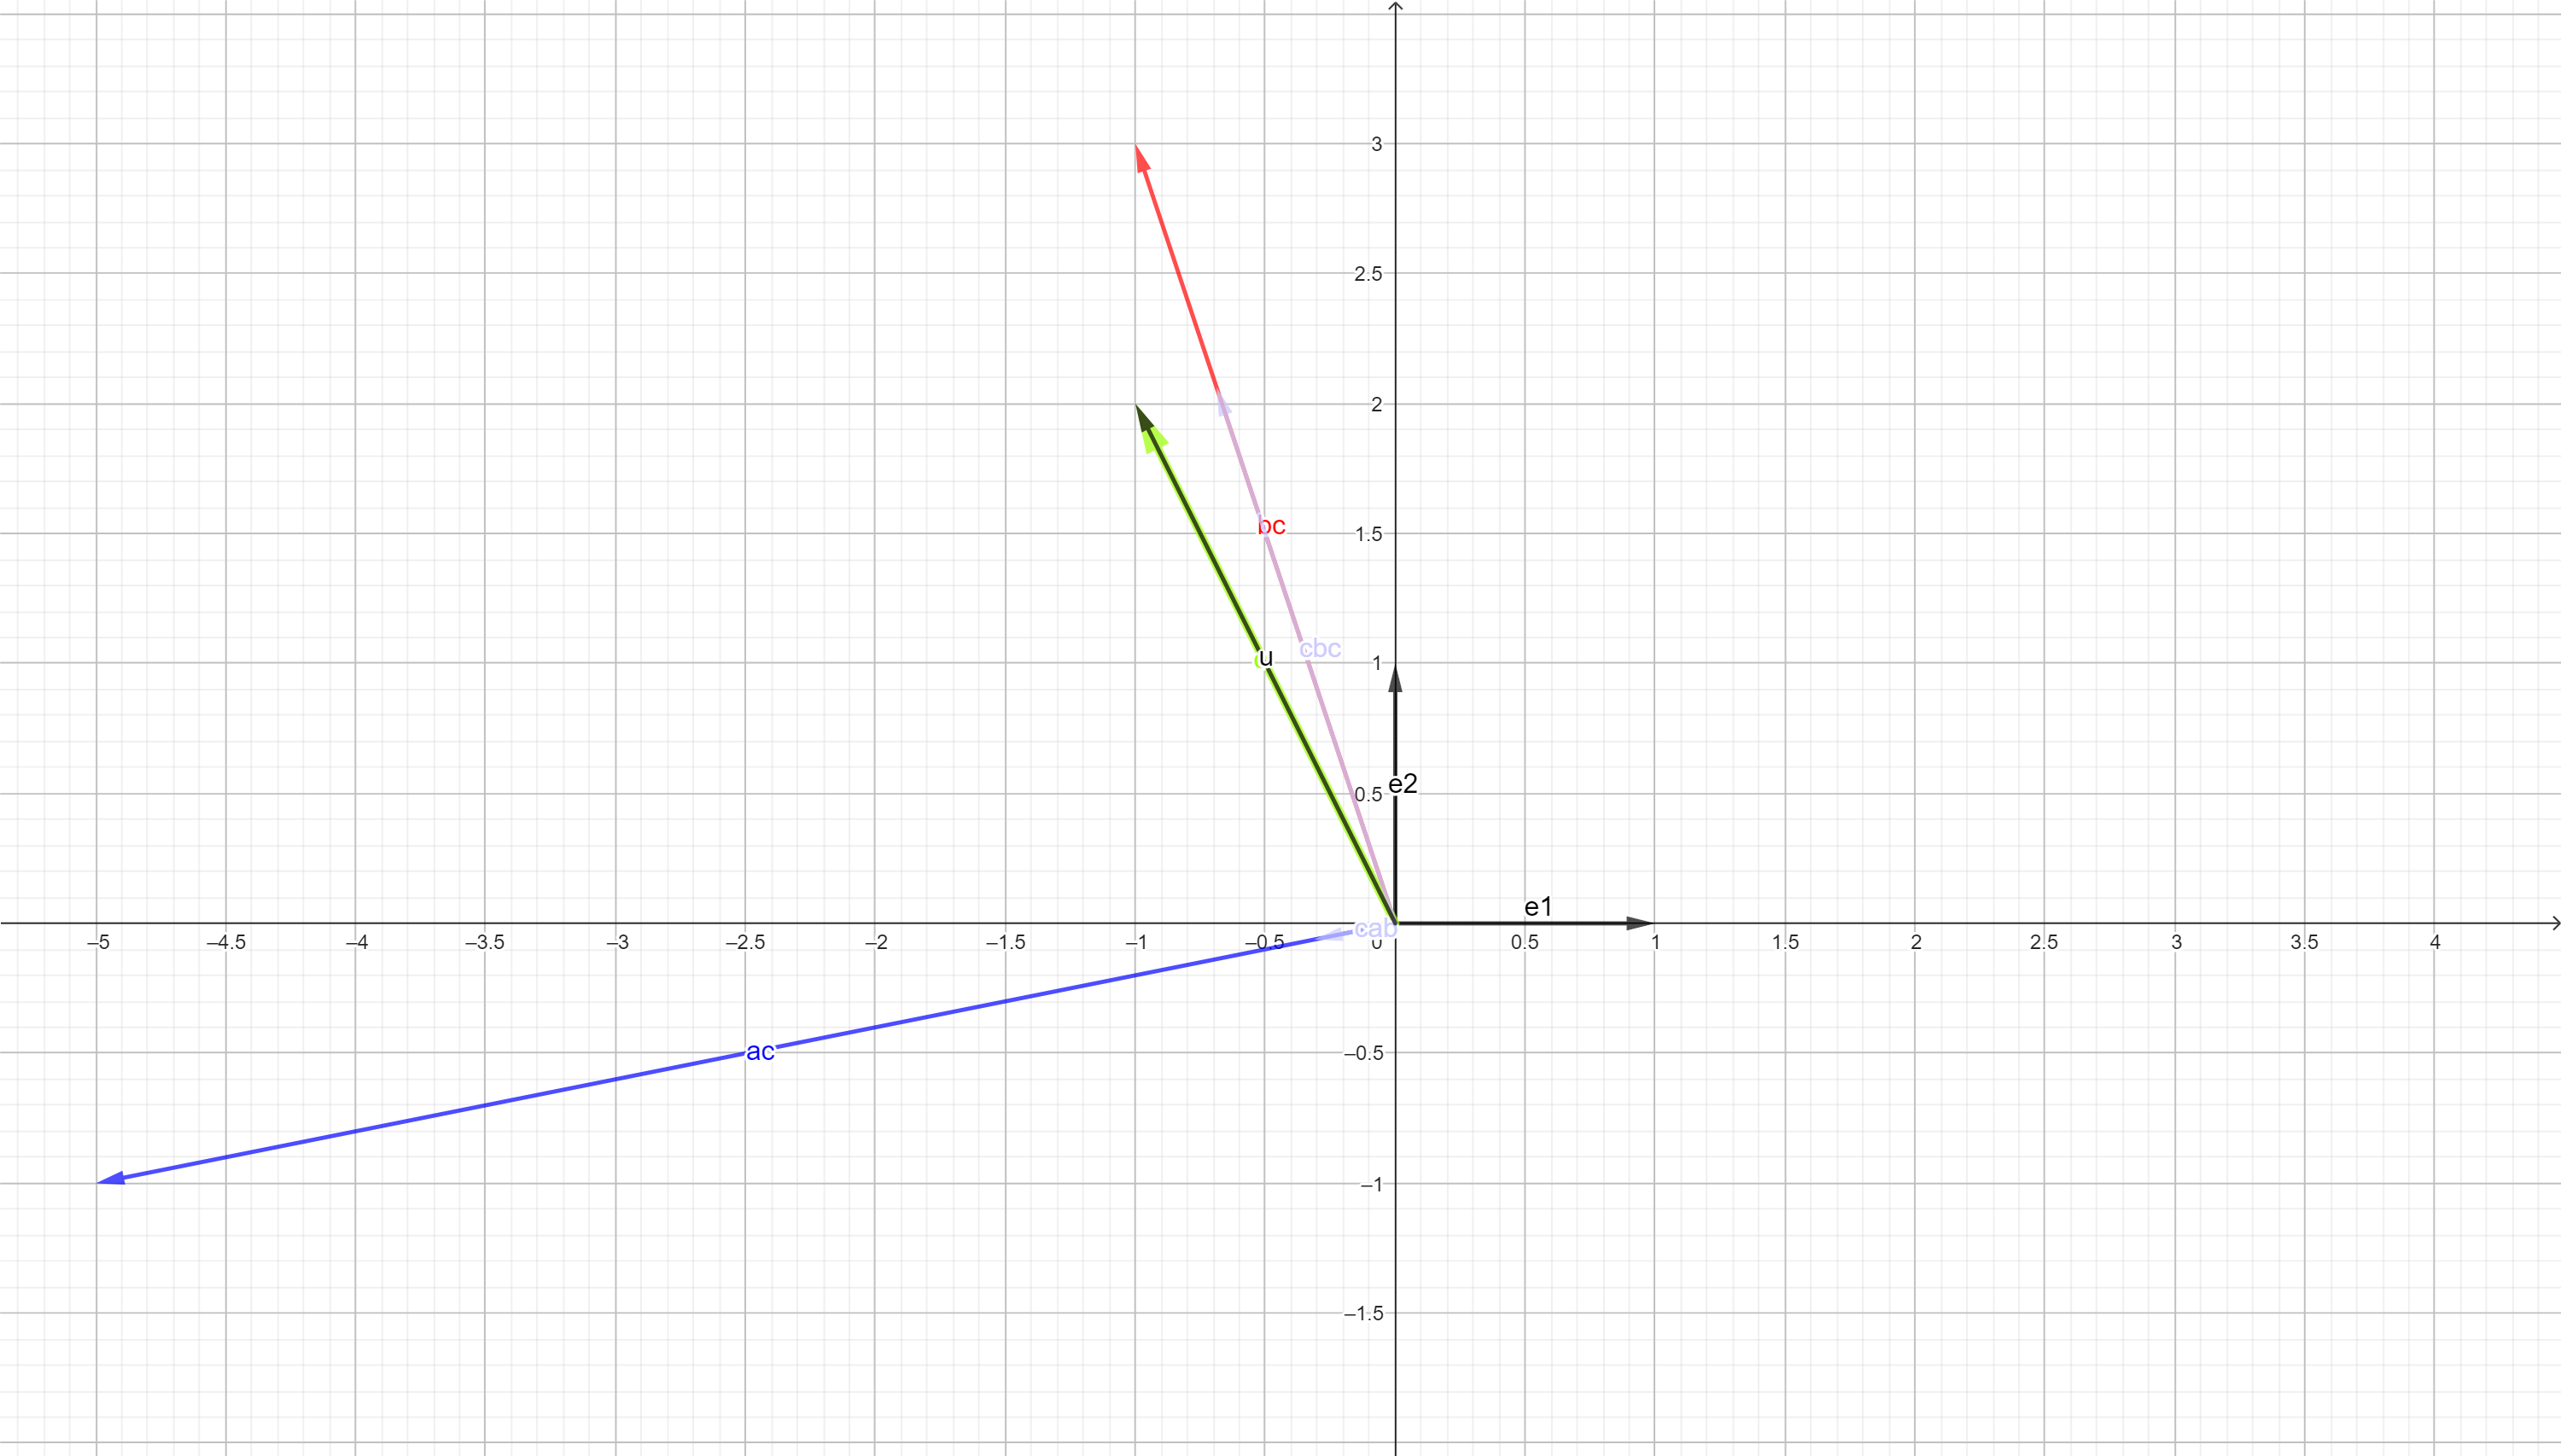
\includegraphics[height=6cm,width=1\textwidth,keepaspectratio]{resources/lab4_t3.png}}
            \label{fig:resources/lab4_t3.png}
        \end{figure}
    }
\end{frame}


\begin{frame}[t]{Changing Basis}
    \framesubtitle{Task 4}
    \only<1>{
    Two bases are given in the plane: $\textbf{e}_1$, $\textbf{e}_2$ and $\textbf{e}'_1$, $\textbf{e}'_2$. The vectors of the second basis have coordinates $(-1;\,3)$ and $(2;-7)$ in the first basis.

    (a) Compose transition matrices from the old basis to the new and vice versa.

    (b) Find the coordinates of a vector in the old basis given that it has coordinates $\alpha'_1$, $\alpha'_2$ in the new basis.

    (c) Find the coordinates of a vector in the new basis given that it has coordinates $\alpha_1$, $\alpha_2$ in the old basis.}
    \only<2>{\alert{\Large Answer}
    
    \begin{align*}
        E = \begin{bmatrix} \vec{e}_1 &\vec{e}_2 \end{bmatrix},\ E = \begin{bmatrix} \vec{e'}_1 & \vec{e'}_2 \end{bmatrix} \\
        E\begin{bmatrix} -1\\ 3 \end{bmatrix} = E'\begin{bmatrix} 1\\ 0 \end{bmatrix},\ E\begin{bmatrix} 2\\ -7 \end{bmatrix}=E'\begin{bmatrix} 0\\ 1 \end{bmatrix} \text{, because its a second basis itself} \\
        \text{combine together} \\
        E\begin{bmatrix}
        -1 & 2\\ 
        3 & -7 
        \end{bmatrix} = E' \begin{bmatrix}
        1 & 0\\ 
        0 & 1 
        \end{bmatrix} \Rightarrow E\underbrace{\begin{bmatrix}
            -1 & 2\\ 
            3 & -7 
            \end{bmatrix}}_{A}=E' 
    \end{align*}}
\end{frame}

\begin{frame}[t]{Changing Basis}
    \framesubtitle{Change the coordinate frame}
    \vspace{-0.6cm}
    \begin{figure}[H]
        \centering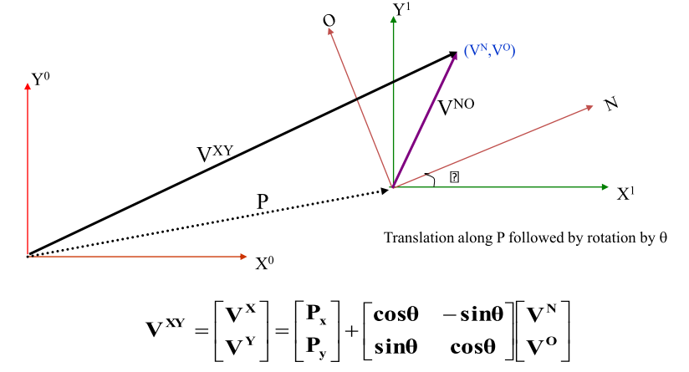
\includegraphics[height=6cm,width=1\textwidth,keepaspectratio]{change_klimchik_1.png}
        % \caption{caption_name}
        \label{fig:change_klimchik_1.png}
    \end{figure}
\end{frame}

\begin{frame}[t]{Changing Basis}
    \framesubtitle{Homogeneous representation}
    \vspace{-0.6cm}
    \begin{figure}[H]
        \centering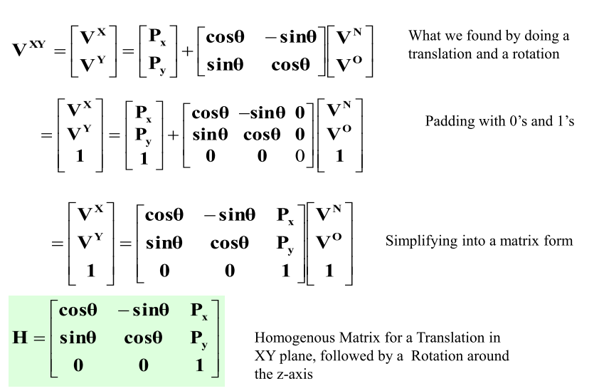
\includegraphics[height=6cm,width=1\textwidth,keepaspectratio]{change_klimchik_2.png}
        % \caption{caption_name}
        \label{fig:change_klimchik_2.png}
    \end{figure}
\end{frame}

\begin{frame}[t]{Changing Basis}
    \framesubtitle{Special Cases of Homogeneous matrices in 3D}
    \vspace{-0.6cm}
    \begin{figure}[H]
        \centering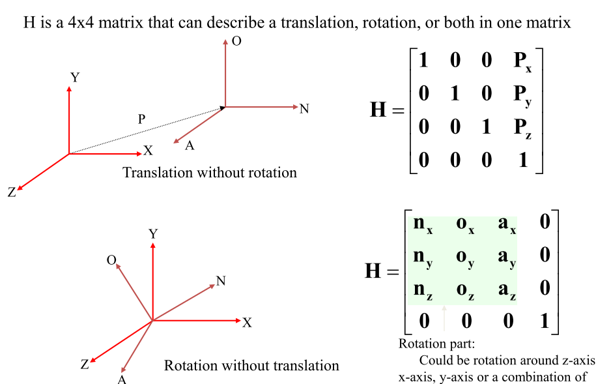
\includegraphics[height=6cm,width=1\textwidth,keepaspectratio]{change_klimchik_3.png}
        % \caption{caption_name}
        \label{fig:change_klimchik_3.png}
    \end{figure}
\end{frame}

\begin{frame}[t]{Changing Basis}
    \framesubtitle{Change the coordinate frame: Case Study}
    \vspace{-0.6cm}
    \begin{figure}[H]
        \centering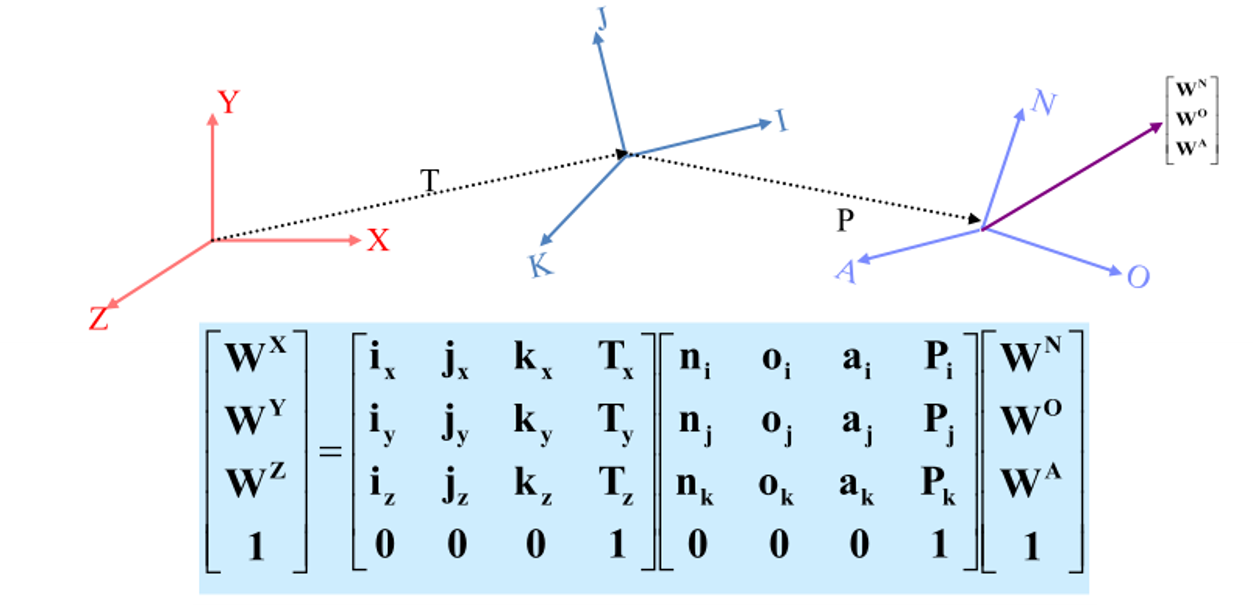
\includegraphics[height=6cm,width=1\textwidth,keepaspectratio]{change_klimchik_4.png}
        % \caption{caption_name}
        \label{fig:change_klimchik_4.png}
    \end{figure}
\end{frame}

\begin{frame}[t]{Changing Basis}
    \framesubtitle{Task 5}
    \only<1>{
    Let us consider two coordinate systems in the plane: $O$, $\textbf{e}_1$, $\textbf{e}_2$ and $O'$, $\textbf{e}'_1$, $\textbf{e}'_2$. Point $O'$ has coordinates $(7;-2)$ in the old coordinate system, and vectors $\textbf{e}'_1$, $\textbf{e}'_2$ can be obtained from vectors $\textbf{e}_1$, $\textbf{e}_2$ by rotating them $60^{\circ}$ (a) clockwise; (b) counterclockwise. Find the old coordinates of a point $x$, $y$ given its new coordinates $x'$, $y'$.
    }
    \only<2>{
        \alert{\Large Answer}

        \begin{align*}
            \text{Classical way, using Extended 2nd Bro eqn} \\
            \begin{bmatrix} x\\ y \end{bmatrix} = \begin{bmatrix} 7\\ -2 \end{bmatrix} + \begin{bmatrix}
            \cos 60 & -\sin 60\\ 
            \sin 60 & \cos 60 
            \end{bmatrix}\begin{bmatrix} x'\\ y' \end{bmatrix} \\
            \text{Or using Homogeneous matrix}\\
            \begin{bmatrix} x\\ y \\ 1 \end{bmatrix} = \begin{bmatrix}
            \cos 60 & -\sin 60  & 7 \\
            \sin60 & \cos 60 & -2 \\ 
            0 & 0  & 1 
            \end{bmatrix}\begin{bmatrix} x'\\ y' \\1\end{bmatrix}
        \end{align*}
    }
\end{frame}


\begin{frame}[t]{Changing Basis}
    \framesubtitle{Task 6}
    There are to bases in $R^3$:

    $e_1=i,\ e_2=j,\ e_3=k$ and $e_1'=i+j+k,\ e_2'=i+j,\ e_3'=i$

    Find coordinates of $x=2i-3j+k$ in the basis $e_1',\ e_2',\ e_3'$.
\end{frame}



\begin{frame}[t]{Changing Basis}
    \framesubtitle{Task 7}
    There are 4 vectors $f_1,\ f_2,\ f_3,\ x$ and the basis \\ $e_1=\begin{bmatrix}1\\0\\0\end{bmatrix},\ e_2=\begin{bmatrix}0\\1\\0\end{bmatrix},\ e_3=\begin{bmatrix}0\\0\\1\end{bmatrix}$. Find the coordinates of $x$ in the basis $(f_1,\ f_2,\ f_3)$, if $f_1=\begin{bmatrix}1\\1\\1\end{bmatrix},\ f_2=\begin{bmatrix}1\\2\\1\end{bmatrix},\ f_3=\begin{bmatrix}1\\2\\2\end{bmatrix},\ x=\begin{bmatrix}1\\1\\0\end{bmatrix}$
\end{frame}

\begin{frame}[t]{Reference material}
    % \framesubtitle{OnlineMschool}
    \Large
    \begin{itemize}
        \item \href{https://onlinemschool.com/math/library/matrix/inverse/}{Inverse Matrix (OnlineMschool)}
        \item \href{https://en.wikipedia.org/wiki/Gaussian_elimination}{Gauss-Jordan (Wiki)}
        \item \href{https://www.youtube.com/watch?v=P2LTAUO1TdA}{Changing Basis (3Blue1Brown)}
    \end{itemize}
\end{frame}

\fbckg{fibeamer/figs/last_page.png}
\frame[plain]{}

\usebackgroundtemplate{}
\setbeamercolor{background canvas}{bg=}
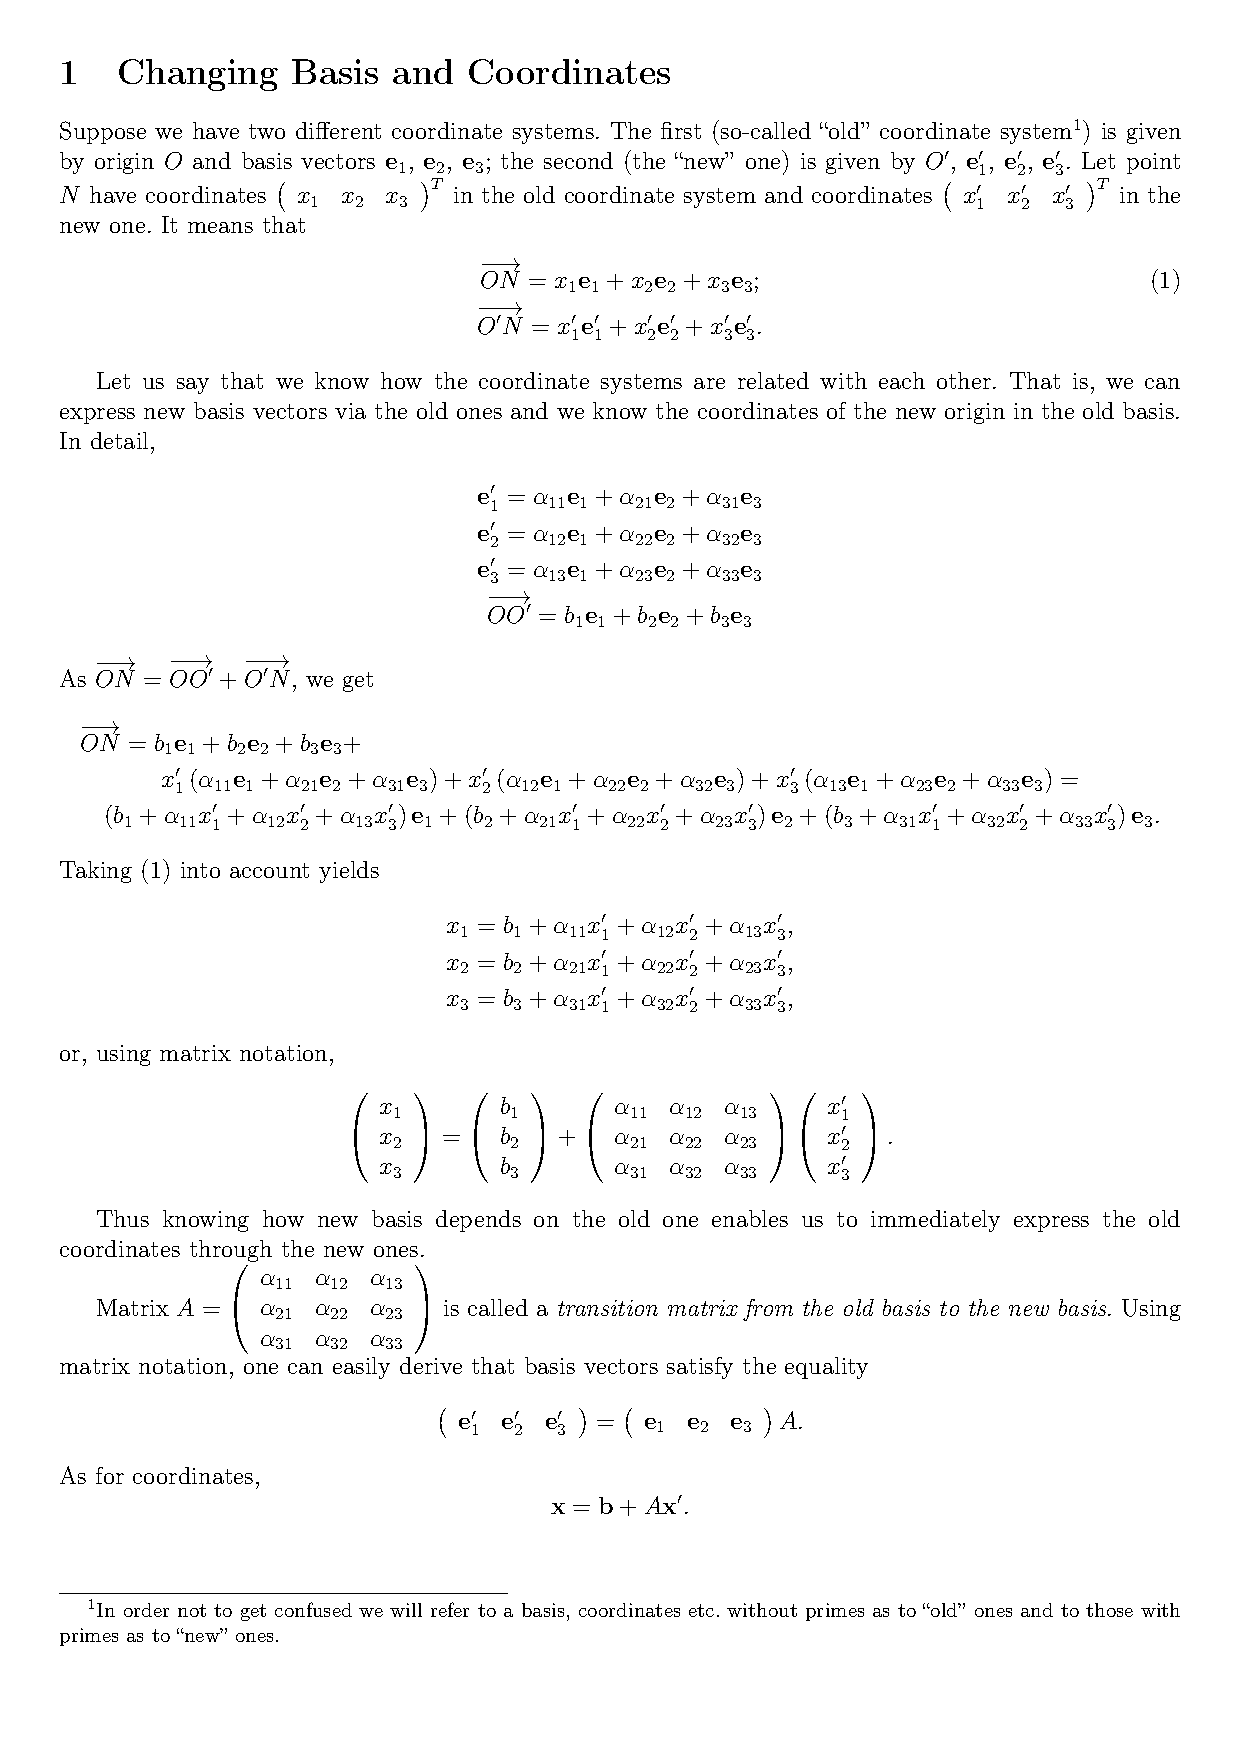
\includepdf[pages=-,fitpaper, linktodoc=true, pagecommand={\section{My header}\label{pdf:myfile}}]{change_of_basis_gorodetskii.pdf}

\fbckg{fibeamer/figs/common.png}

\end{document}